%% Преамбула TeX-файла

% 1. Стиль и язык
\documentclass[utf8x]{G7-32} % Стиль (по умолчанию будет 14pt)
\usepackage[T2A]{fontenc}
\usepackage[russian]{babel}

% Остальные стандартные настройки убраны в preamble.inc.tex.
\sloppy

% Настройки стиля ГОСТ 7-32
% Для начала определяем, хотим мы или нет, чтобы рисунки и таблицы нумеровались в пределах раздела, или нам нужна сквозная нумерация.
\EqInChapter % формулы будут нумероваться в пределах раздела
\TableInChapter % таблицы будут нумероваться в пределах раздела
\PicInChapter % рисунки будут нумероваться в пределах раздела

% Добавляем гипертекстовое оглавление в PDF
\usepackage[
bookmarks=true, colorlinks=true, unicode=true,
urlcolor=black,linkcolor=black, anchorcolor=black,
citecolor=black, menucolor=black, filecolor=black,
]{hyperref}

% Изменение начертания шрифта --- после чего выглядит таймсоподобно.
% apt-get install scalable-cyrfonts-tex

\IfFileExists{cyrtimes.sty}
    {
        \usepackage{cyrtimespatched}
    }
    {
        % А если Times нету, то будет CM...
    }

\usepackage{graphicx}   % Пакет для включения рисунков

% С такими оно полями оно работает по-умолчанию:
% \RequirePackage[left=20mm,right=10mm,top=20mm,bottom=20mm,headsep=0pt]{geometry}
% Если вас тошнит от поля в 10мм --- увеличивайте до 20-ти, ну и про переплёт не забывайте:
\geometry{right=20mm}
\geometry{left=30mm}


% Пакет Tikz
\usepackage{tikz}
\usetikzlibrary{arrows,positioning,shadows}

% Произвольная нумерация списков.
\usepackage{enumerate}

% ячейки в несколько строчек
\usepackage{multirow}

% itemize внутри tabular
\usepackage{paralist,array}

\usepackage{natbib}

\bibliographystyle{apalike}
\bibpunct{[}{]}{,}{a}{}{;}

\usepackage{tabulary}
\usepackage{caption}



% Настройки листингов.
% 8 Листинги

\usepackage{listings}

% Значения по умолчанию
\lstset{
  basicstyle= \footnotesize,
  breakatwhitespace=true,% разрыв строк только на whitespacce
  breaklines=true,       % переносить длинные строки
%   captionpos=b,          % подписи снизу -- вроде не надо
  inputencoding=koi8-r,
  numbers=left,          % нумерация слева
  numberstyle=\footnotesize,
  showspaces=false,      % показывать пробелы подчеркиваниями -- идиотизм 70-х годов
  showstringspaces=false,
  showtabs=false,        % и табы тоже
  stepnumber=1,
  tabsize=4,              % кому нужны табы по 8 символов?
  frame=single
}

% Стиль для псевдокода: строчки обычно короткие, поэтому размер шрифта побольше
\lstdefinestyle{pseudocode}{
  basicstyle=\small,
  keywordstyle=\color{black}\bfseries\underbar,
  language=Pseudocode,
  numberstyle=\footnotesize,
  commentstyle=\footnotesize\it
}

% Стиль для обычного кода: маленький шрифт
\lstdefinestyle{realcode}{
  basicstyle=\scriptsize,
  numberstyle=\footnotesize
}

% Стиль для коротких кусков обычного кода: средний шрифт
\lstdefinestyle{simplecode}{
  basicstyle=\footnotesize,
  numberstyle=\footnotesize
}

% Стиль для BNF
\lstdefinestyle{grammar}{
  basicstyle=\footnotesize,
  numberstyle=\footnotesize,
  stringstyle=\bfseries\ttfamily,
  language=BNF
}

% Определим свой язык для написания псевдокодов на основе Python
\lstdefinelanguage[]{Pseudocode}[]{Python}{
  morekeywords={each,empty,wait,do},% ключевые слова добавлять сюда
  morecomment=[s]{\{}{\}},% комменты {а-ля Pascal} смотрятся нагляднее
  literate=% а сюда добавлять операторы, которые хотите отображать как мат. символы
    {->}{\ensuremath{$\rightarrow$}~}2%
    {<-}{\ensuremath{$\leftarrow$}~}2%
    {:=}{\ensuremath{$\leftarrow$}~}2%
    {<--}{\ensuremath{$\Longleftarrow$}~}2%
}[keywords,comments]

% Свой язык для задания грамматик в BNF
\lstdefinelanguage[]{BNF}[]{}{
  morekeywords={},
  morecomment=[s]{@}{@},
  morestring=[b]",%
  literate=%
    {->}{\ensuremath{$\rightarrow$}~}2%
    {*}{\ensuremath{$^*$}~}2%
    {+}{\ensuremath{$^+$}~}2%
    {|}{\ensuremath{$|$}~}2%
}[keywords,comments,strings]

% Подписи к листингам на русском языке.
\renewcommand\lstlistingname{\cyr\CYRL\cyri\cyrs\cyrt\cyri\cyrn\cyrg}
\renewcommand\lstlistlistingname{\cyr\CYRL\cyri\cyrs\cyrt\cyri\cyrn\cyrg\cyri}


% Полезные макросы листингов.
% Любимые команды
\newcommand{\Code}[1]{\textbf{#1}}


\begin{document}

\frontmatter % выключает нумерацию ВСЕГО; здесь начинаются ненумерованные главы: реферат, введение, глоссарий, сокращения и прочее.

% Команды \breakingbeforechapters и \nonbreakingbeforechapters
% управляют разрывом страницы перед главами.
% По-умолчанию страница разрывается.

% \nobreakingbeforechapters
% \breakingbeforechapters

% Также можно использовать \Referat, как в оригинале
\begin{abstract}
В данной работе исследована возможность использования се\-ман\-ти\-ко-син\-так\-си\-чес\-ко\-го
анализатора Compreno в качестве источника высокоуровневых признаков
для решения задачи распознавания именованных сущностей в рамках нейросетевого подхода.
Исследование проводилось на англоязычном корпусе CoNLL 2003.
Полученные результаты показывают, что высокоуровневые признаки
дают ощутимый прирост оценки качества, без какой-либо инженерии над ними.

\smallskip
\noindent \textbf{Ключевые слова:} нейронные сети, распознавание именованных сущностей.
\end{abstract}

%%% Local Variables:
%%% mode: latex
%%% TeX-master: "rpz"
%%% End:


\tableofcontents
% Введение
% Обзор литературы
% Теоретическое исследование
% Практическое исследование

\Defines
\begin{description}
\item[Функция потерь] функция, которая минимизируется при оптимизации модели. Она представляет выбранную меру несогласия наблюдаемых данных и данных, предсказываемых подогнанной функцией.
\item[Дискриминативные модели] семейство моделей, восстанавливающих апостериорную вероятность.
\item[Инженерия признаков] вручную построенные признаки, инженерный подход к построению признаков.
\item[Векторное представление слова] сопоставление словам некоторых непрерывных векторов из множества вещественных чисел.
\item [Именованная сущность] слово или словосочетание обозначающее предмет или явления определенной категории.
\item[Распознавание именованных сущностей] (named entity recognition, NER) выделение и классификация именованных сущностей в тексте.
\end{description}

%%% Local Variables:
%%% mode: latex
%%% TeX-master: "rpz"
%%% End:

\Abbreviations %% Список обозначений и сокращений в тексте
\begin{description}
\item[NER] Named Entity Recognition.
\end{description}

%%% Local Variables:
%%% mode: latex
%%% TeX-master: "rpz"
%%% End:


\Introduction

  Именованная сущность - это слово или словосочетание обозначающее
  предмет или явления определенной категории. Примерами именованных сущностей
  являются имена людей, названия организаций и локаций.
  Задача распознавания именованных сущностей (Named Entity Recognition, NER)
  состоит в выделении и классификация именованных сущностей в тексте.
  В рамках конференции CoNLL 2003 проводилось соревнование
  для оценки качества методов распознавания именованных сущностей четырех типов
  на англоязычном корпусе \citep{tjong2003introduction}.
  Для решения задачи NER предлагалось много разных подходов \citep{nadeau2007survey}.
  В последнее время было показано, что методы на основе нейронных сетей показывают
  лучшие результаты для различных языков и корпусов, включая CoNLL 2003 \citep{DBLP:journals/corr/YangSC16}.

  Вместо большого количества вручную построенных признаков
  решающих определенную задачу, нейросетевые методы используют универсальные
  векторные представления слов \citep{mikolov2013distributed}.
  Согласно гипотезе о дистрибутивности, эти представления
  кодируют в себе смысл слов \citep{sahlgren2008distributional}.
  Это позволяет строить мультизадачные и языконезависимые
  архитектуры \citep{collobert2011natural, DBLP:journals/corr/YangSC16}.

  Несмотря на то, что использование универсальных векторных представлений
  получило в последнее время огромную популярность в силу своей эффективности
  и огромной экономии человеческих усилий, большой интерес все еще представляет
  исследование возможностей использования высокоуровневых признаков
  в качестве входных данных для нейросетей.
  Так, например, в работах \citep{xu2014rc, bian2014knowledge} описано использование
  морфологических, синтаксических и семантических признаков для построения
  более совершенных векторных представлений слов.

  Compreno -  это технология автоматического анализа текстов на естественном языке,
  в основе которой
  лежит многоуровневое лингвистическое описание, создававшееся профессиональными
  лингвистами в течение длительного времени \citep{anisimovich2012syntactic}.
  Помимо ручного описания Compreno использует для анализа большое количество
  информации, извлекаемых различными статистическими методами из текстовых корпусов.
  В Compreno реализована процедура семантико-синтаксического анализа текста,
  в результате которой любому предложению на естественном языке (английском или русском)
  ставится в соответствие семантико-синтаксическое дерево, моделирующее смысл предложения
  и содержащее грамматическую и семантическую информацию о каждом слове предложения.

  В данной работе исследована возможность использования семантико-синтаксического
  анализатора Compreno в качестве источника высокоуровневых признаков для задачи
  NER на корпусе CoNLL 2003 в рамках нейросетевого подхода.

  Статья организована следующим образом: в части 1 проведен обзор связанных работ.
  Выбранная нейросетевая модель и способы внедрения синтактико-семантических признаков описаны в части 2.
  В части 3 описаны проведенные эксперименты и программная реализация.

  Полученные результаты показывают повышение F1-меры почти на 1\% на корпусе CoNLL 2003
  при использовании синтактико-семантических признаков Compreno (87.49\% против 88.47\%).
  При этом затраты на их внедрение были минимальными - инженерия над признаками не проводилась.


\mainmatter % это включает нумерацию глав и секций в документе ниже

\chapter{Обзор литературы}

Победители соревнования по NER CoNLL 2003 \citep{florian2003named}, получившие 88.76\% F1,
представили систему использующую комбинацию различных алгоритмов машинного обучения.
В качестве признаков был использован их собственный, вручную составленный газетир,
POS-теги, CHUNK-теги, суффиксы, префиксы и выход других NER-классификаторов,
тренированных на внешних данных.

\citep{collobert2011natural} представили комбинацию сверточной нейронной сети
с условными случайными полями, получившую 89.59\% F1 на корпусе CoNLL 2003.
Их нейросетевая архитектура не зависит от задачи и используется как для NER, так и для
частеречной разметки (part-of-speech tagging), поиска синтаксически связанных групп
соседних слов (chunking), установления семантических ролей (semantic role labelling).
Для задачи NER они использовали три типа признаков - векторное представление слова,
капитализацию и небольшой газетир, включенный в соревнование CoNLL 2003.

\citep{chiu2015named} представили комбинацию сверточных сетей, рекуррентных сетей
и условных случайных полей.
Они использовали такие же признаки как у \citep{collobert2011natural}, дополнительный, вручную сформированный
газетир на основе DBpedia и обучались на
train+dev\footnote{Объединенная обучающая и валидационная выборки} выборке CoNLL 2003.
У них получилось 91.62\% F1. Кроме корпуса CoNLL 2003 они тестировали архитектуру
на более крупном англоязычном корпусе OntoNotes 5.0. На нем они получили
state-of-the-art результат 86.28\%.

\citep{DBLP:journals/corr/YangSC16} представили глубокую иерархическую рекуррентную нейросетевую
архитектуру с условными случайными полями для разметки последовательностей.
Они использовали такие же признаки как у \citep{collobert2011natural}.
Кроме англоязычного корпуса CoNLL 2003, где они получили state-of-the-art 90.94\% F1 при обучении
только на обучающей выборке (train set), они тестировали работу нейросети на CoNLL 2002 Dutch NER и CoNLL 2003 Spanish NER.
На этих корпусах они улучшили предыдущий state-of-the-art результат:
82.82\% до 85.19\% на CoNLL 2002 Dutch NER и 85.75\% до 85.77\% на CoNLL 2003 Spanish NER.

Современные работы используют векторное представление слов
и условные случайные поля в своих моделях. Из сторонних признаков применяют
только газетиры. В работах \citep{xu2014rc, bian2014knowledge} описано применение дополнительных признаков для
слов (морфологических, синтаксических, семантических) для создания более
совершенных векторных представлений.
Такие векторные представления помогают повысить оценку качества в
прикладных задачах \citep{xu2014rc}.


\chapter{Теоретическая часть}
\section{Модель}

  Для реализации была выбрана сверточная нейронная сеть из статьи \citep{collobert2011natural}.
  Из модели были удалены условные случайные поля для более быстрого обучения и проведения экспериментов.

  В качестве признаков выступают вектора слов, позиция относительно слова в предложении
  для которого предсказывается тег, капитализация и присутствие слова в газетире,
  который включен в соревнование CoNLL 2003.

  Общий алгоритм работы следующий:
  \begin{enumerate}
    \item В начало и конец предложения добавляют по одному специальному токену, чтобы его длина была
    не меньше трех. Каждый токен отображается в набор идентификаторов признаков.
    На вход нейросети поступает набор идентификаторов признаков для всего предложения.

    \item Набор идентификаторов пропускается через специальный слой (lookup table), который отображает
    каждый идентификатор в вектор весов. На выходе каждому токену предложения соответствует
    вектор.
    \item Полученные вектора объединяются в матрицу признаков предложения.
    \item Полученная матрица признаков подается на следующий
    слой, который проходится окном размера 3 и выполняет операцию свертки (temporal convolution).
    Т.е. три столбца матрицы признаков конкатенируются в один вектор и перемножаются
    на матрицу весов справа.
    На выходе получается матрица с количеством строк фиксированной длины (для любого предложения).
    \item Затем извлекается максимум по каждой строке (max over time).
    Таким образом все предложения любой длины получают вектор признаков фиксированной длины.
    \item Полученный вектор признаков подается на полносвязный слой.
    \item Затем выход полносвязного слоя подается на выходной слой, который возвращает вероятность
    для каждого тега (softmax).
  \end{enumerate}

  В качестве функции потерь используется кросс-энтропия (cross entropy).

  Подробная математическая модель описана в статье \citep{collobert2011natural}.

  \subsection{Синтактико-семантические признаки}
    Существует много инструментов для получения дополнительных признаков для слова.
    Для извлечения синтаксических признаков часто используют MaltParser \citep{nivre2006maltparser}.
    Для получения семантических признаков применяют BabelNet \citep{navigli2010babelnet}.

    В данной работе для получения синтактико-семантических признаков используется Compreno.
    Вершины синтактико-семантического дерева Compreno кодировались бинарным представлением
    и соотносились с токенами исходного
    текста\footnote{Почти для всех токенов в соответствующем дереве нашлась соответствующая вершина.
    Токены для которых не была найдена вершина, кодировались специальным признаком 83951},
    тем самым наделяя их синтактико-се\-ман\-ти\-ческими признаками.
    Размерность пространства синтактико-се\-ман\-ти\-ческих признаков получилась равной 83950.

    Плотные вектора большой размерности сильно замедляют процесс оптимизации и для хорошего
    обучения требуется много данных и вычислительных ресурсов.
    В таких случаях часто применяют методы для уменьшения размерности,
    например сингулярное разложение или автоэнкодеры. Минусом таких методов является потеря информации
    после сжатия.

    Если же вектора большой размерности разреженные, то используют специальные методы для
    работы с такими данными \citep{davissurvey}.

    В данной работе предлагается 2 способа внедрения синтактико-семантических признаков:
    \begin{itemize}
      \item сжать синтактико-семантические вектора с помощью сингулярного разложения (SVD) и добавить
      как еще один Lookup Table в сверточную нейронную сеть;
      \item добавить еще одну нейронную сеть для синтактико-семантических признаков и оптимизировать
      её вместе со сверточной нейронной сетью.
    \end{itemize}


\chapter{Экспериментальная часть}

\section{Корпус CoNLL 2003}

CoNLL 2003 \citep{tjong2003introduction} - англоязычный корпус для оценки качества
методов распознавания именованных сущностей.
Корпус содержит обучающую, тестовую и валидационную выборку.
Размечено 4 типа сущностей - персоны (PER), организации (ORG), локации (LOC) и другие (MISC).
Корпус размечен по схеме Inside, Outside, Begin (IOB).
Оценка качества считается с помощью F1-micro-average.

\begin{table}[ht]
  \caption{Количество статей, предложений, токенов и именованных сущностей}
  \centering
  \begin{tabular}{ | p{3cm} | p{1.5cm} | p{2.5cm} | p{1.5cm} | p{1cm} | p{1cm} | p{1cm}| p{1cm} |}
    \hline\hline
    Выборка & Статьи & Предложения & Токены & LOC & MISC & ORG & PER \\
    \hline
    Обучающая & 946 & 14987 & 203621 & 7140 & 3438 & 6321 & 6600 \\
    \hline
    Валидационная & 216 & 3466 & 51362 & 1837 & 922 & 1341 & 1842 \\
    \hline
    Тестовая & 231 & 3684 & 46435 & 1668 & 702 & 1661 & 1617 \\
    \hline
  \end{tabular}
\end{table}

Как и у \citep{collobert2011natural}, данные были сконвертированы из схемы IOB
в схему IOBES (Inside, Outside, Begin, End, Single).
Во время тестирования, данные конвертируются обратно в формат IOB и подаются на вход скрипта,
включенного в CoNLL 2003, оценивающего качество классификации.

\section{Синтактико-семантические признаки Compreno}
Синтактико-семантически признаки были получены с помощью Compreno.
Они представляют собой разреженные вектора размерности 83950.
Они покрывают около 60\% корпуса CoNLL 2003.
Все токены, не покрытые Compreno, кодировались как дополнительный признак 83951.

\section{Эксперименты без синтактико-семантических признаков}

Нейросетевая модель имеет такие же параметры как и у \citep{collobert2011natural}.
Небольшой модификацией является добавление Dropout слоя в качестве регуляризатора,
после каждого полносвязного слоя.
Размерность выходного слоя - 17. Четыре для каждого из четырех типов тегов и один для Outside.

В качестве векторного представления слов (embeddings в таблице \ref{table:raw_net}),
использовались Senna embeddings\footnote{http://ronan.collobert.com/senna/},
которые находятся в открытом доступе.
\newpage
\begin{table}[!h]
  \caption{Результаты экспериментов без использования синтактико-семантических признаков}
  \centering
  \begin{tabulary}{\textwidth}{| L | L | L | L | L | L |}
    \hline\hline
    \multicolumn{1}{|p{1.5cm}|}{Модель} & Признаки & Выборка & Метод оптимизации & Полученная F1, \% & F1 в статье \cite{collobert2011natural} \\
    \hline
    Window & Embeddings, Capitalization & train & Mini-batch gradient descent & 86.27 & - \\
    \hline
    Window & Embeddings, Capitalization & train & Stochastic gradient descent & - & 86.97 \\
    \hline
    ConvNet + CRF & Embeddings, Capitalization, Position & train & Stochastic gradient descent & - & 88.67 \\
    \hline
    ConvNet + CRF & Embeddings, Capitalization, Position, Gazetteer & train & Stochastic gradient descent & - & 89.59 \\
    \hline
    ConvNet & Embeddings, Capitalization, Position & train & Stochastic gradient descent & 86.77 & - \\
    \hline
    ConvNet & Embeddings, Capitalization, Position, Gazetteer & train & Stochastic gradient descent & 87.89 & - \\
    \hline
    ConvNet & Embeddings, Capitalization, Position, Gazetteer & train + dev & Stochastic gradient descent & 88.37 & - \\
    \hline
    ConvNet & Embeddings, Capitalization, Position, Gazetteer & train & Mini-batch gradient descent & \textbf{87.49} & - \\
    \hline
  \end{tabulary}
  \label{table:raw_net}
\end{table}

По таблице \ref{table:raw_net} видно, что результаты немного ниже чем у \citep{collobert2011natural}.
Это связано с тем, что для Window подхода использован другой метод оптимизации,
а для Convolution подхода не были применены условные случайные поля.

В качестве референсной, будет использована модель из последнего эксперимента
показывающая 87.49\% F1.
Это сделано для чистоты эксперимента, т.к. далее  обучение происходило только
на обучающей выборке по правилам соревнования CoNLL 2003 и применялся mini-batch
gradient descent для ускорения экспериментов.

\section{Эксперименты с синтактико-семантическими признаками сжатыми с использованием SVD}

Синтактико-семантически признаки Compreno размерности 83950 были сжаты с использованием
TruncatedSVD\footnote{http://scikit-learn.org/stable/modules/generated/sklearn.decomposition.TruncatedSVD.html}
до размерности 1024.
После сжатия описываемая дисперсия была равна 72\%. Т.е. потерялось 28\% информации.
Сжатые вектора были добавлены в нейронную сеть с помощью дополнительного Lookup Table слоя.
\newpage
\begin{table}[!h]
  \caption{Результаты с синтактико-семантическими признаками сжатыми SVD}
  \centering
  \begin{tabulary}{\textwidth}{| L | L | L | L | L | L |}
    \hline\hline
    \multicolumn{1}{|p{1.5cm}|}{Модель} & Признаки & Выборка & Метод оптимизации & Полученная F1, \% \\
    \hline
    ConvNet & Position, Compreno SVD 1024 & train & Mini-batch gradient descent & 75.89 \\
    \hline
    ConvNet & Capitalization, Position, Gazetteer, Compreno SVD 1024 & train & Mini-batch gradient descent & 81.83 \\
    \hline
    ConvNet & Embeddings, Capitalization, Position, Gazetteer, Compreno SVD 1024 & train & Mini-batch gradient descent & 86.85 \\
    \hline
    ConvNet & Embeddings, Capitalization, Position, Gazetteer & train & Mini-batch gradient descent & 87.49 \\
    \hline
  \end{tabulary}
  \label{table:svd_net}
\end{table}


По таблице \ref{table:svd_net} видно, что такой способ ведет к небольшому ухудшению F1-меры.


\section{Эксперименты с синтактико-семантическими признаками для совместно-оптимизированной нейросети}

Была добавлена еще одна нейронная сеть для синтактико-семантических признаков и оптимизирована
вместе со сверточной нейронной сетью.

Нейронная сеть для синтактико-семантических признаков работает следующим образом:
\begin{enumerate}
  \item На вход подается разреженный вектор признаков слова (размерность 83951) для которого предсказывается тег.
  \item Далее этот вектор пропускается через 2 полносвязных слоя.
  \item На выходе еще один полносвязный слой, который выдает вероятность определенного тега.
  Выходов также 17.
\end{enumerate}

Сверточная сеть, учитывающая всё предложение, и полносвязная сеть, обрабатывающая
синтактико-семантические признаки слова для которого предсказывается тег, соединяются следующим
образом (рис. \ref{figure:union_net}):
\begin{enumerate}
  \item Из обеих нейросетей удаляются выходные слои.
  \item Предыдущие слои из обеих сетей соединяются в новый полносвязный слой.
  \item Новый полносвязный слой соединяется с выходным слоем. Выходов как и тегов 17.
\end{enumerate}

\begin{figure}[h]
  \caption{Объединение двух нейросетей}
  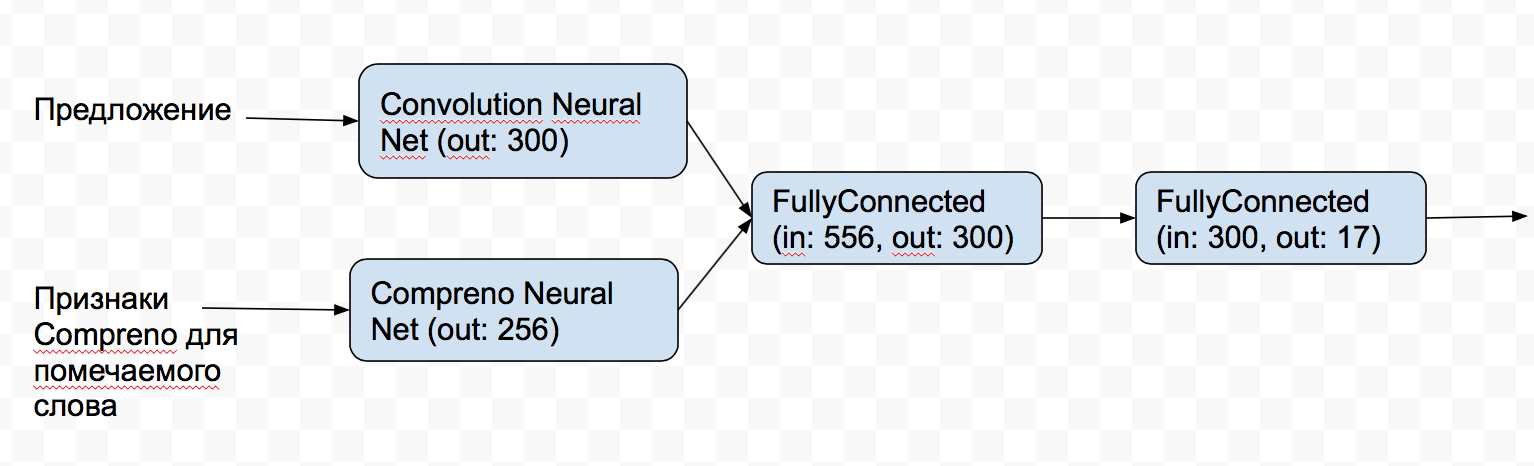
\includegraphics[scale=0.5]{two-net.png}
  \label{figure:union_net}
\end{figure}

Веса у объединенной сети были инициализированы обученными моделями -
моделью показывающую 87.49\% для сверточной сети и моделью показывающую
72.85\% (см. таблицу \ref{table:union_net}) для второй нейронной сети.

\begin{table}[ht]
  \caption{Результаты с синтактико-семантическими признаками для объединенной нейросети}
  \centering
  \begin{tabulary}{\textwidth}{| L | L | L | L | L | L |}
    \hline\hline
    \multicolumn{1}{|p{1.5cm}|}{Модель} & Признаки & Выборка & Метод оптимизации & Полученная F1, \% \\
    \hline
    Compreno Net & Compreno sparse features & train & Mini-batch gradient descent & 72.85 \\
    \hline
    ConvNet & Embeddings, Capitalization, Position, Gazetteer & train & Mini-batch gradient descent & 87.49 \\
    \hline
    ConvNet + Compreno Net & Embeddings, Capitalization, Position, Gazetteer, Compreno sparse features & train & Mini-batch gradient descent & \textbf{88.47} \\
    \hline
    ConvNet + Compreno Net & Embeddings, Capitalization, Position, Gazetteer, Compreno sparse features & train + dev & Mini-batch gradient descent & 88.81 \\
    \hline
  \end{tabulary}
  \label{table:union_net}
\end{table}

По таблице \ref{table:union_net} видно, что признаки Compreno улучшают F1-меру почти на один процент.


\chapter{Программная часть}

Нейронная сеть написана с использованием открытого фреймворка torch\footnote{http://torch.ch}.

Код для воспроизведения экспериментов выложен по адресу:
\href{https://github.com/sld/torch-conv-ner}{github.com/sld/torch-conv-ner}.

Скорость обучения на машине с GPU Amazon AWS g2.2xlarge\footnote{https://aws.amazon.com/ru/ec2/instance-types/}:
\begin{itemize}
\item 1 эпоха при одиночной обработке (stochastic gradient descent): $\sim$450 сек.
\item 1 эпоха при пакетной обработке (mini-batch gradient descent): $\sim$171 сек.
\item Модель получающая 87.49\% обучалась 91 эпоху ($\sim$4.2 часа).
\item 1 эпоха при пакетной обработке с использованием признаков Compreno: $\sim$615 сек.
\end{itemize}

Скорость классификации составляет 2500 токенов в секунду при пакетной обработке.


\backmatter %% Здесь заканчивается нумерованная часть документа и начинаются ссылки и
            %% заключение

\Conclusion % заключение к отчёту

В данной работе исследована возможность использования семантико-синтаксического
анализатора Compreno в качестве источника высокоуровневых признаков для задачи
NER на корпусе CoNLL 2003 в рамках нейросетевого подхода.
Удалось найти простой вариант подключения признаков Compreno к сверточной нейронной
сети за счет которого F1-мера повысилась с 87.49\% до 88.47\%.

В будущем планируется внедрить условные случайные поля в существующую модель для
повышения F1-меры и исследовать работу предложенного решения на других корпусах.
Также интересным направлением для исследований является создание
векторных представлений слов с учетом синтактико-семантических признаков.


%%% Local Variables:
%%% mode: latex
%%% TeX-master: "rpz"
%%% End:


% % Список литературы при помощи BibTeX
% Юзать так:
%
% pdflatex rpz
% bibtex rpz
% pdflatex rpz

\bibliographystyle{gost780u}
\bibliography{rpz}

%%% Local Variables: 
%%% mode: latex
%%% TeX-master: "rpz"
%%% End: 


\appendix   % Тут идут приложения

\cleardoublepage
% \phantomsection
\addcontentsline{toc}{chapter}{\listfigurename}
\listoffigures

%%% Local Variables:
%%% mode: latex
%%% TeX-master: "rpz"
%%% End:

\chapter{Еще картинки}
\label{cha:appendix2}

\begin{figure}
\centering
\caption{Еще одна картинка, ничем не лучше предыдущей. Но надо же как-то заполнить место.}
\end{figure}

%%% Local Variables: 
%%% mode: latex
%%% TeX-master: "rpz"
%%% End: 


\end{document}

%%% Local Variables:
%%% mode: latex
%%% TeX-master: t
%%% End:
